% filepath: /home/sagan/TemplateDissertacaoUnB/README.tex
\documentclass[a4paper,12pt]{article}
\usepackage[utf8]{inputenc}
\usepackage{hyperref}
\usepackage{amsmath, amssymb}
\usepackage[margin=0.5cm]{geometry}
\usepackage{pdfpages}

\title{Template para Dissertação de Mestrado da UnB}
\author{}
\date{}

\begin{document}

\maketitle

\section*{Introdução}

Este documento contém instruções para trabalhar com um template para dissertações de mestrado/teses de doutorado da Universidade de Brasília (UnB), que é um fork do \href{https://github.com/deividrvale/unb-thesis-template}{template feito pelo ex-aluno Deivid Vale}. Abaixo estão descrições detalhadas dos arquivos \texttt{.tex} e como modificá-los para atender a necessidades específicas. Para remover essas instruções do PDF principal, remova (ou comente) a linha 253 de \texttt{thesis.tex}, a saber,
\begin{verbatim}
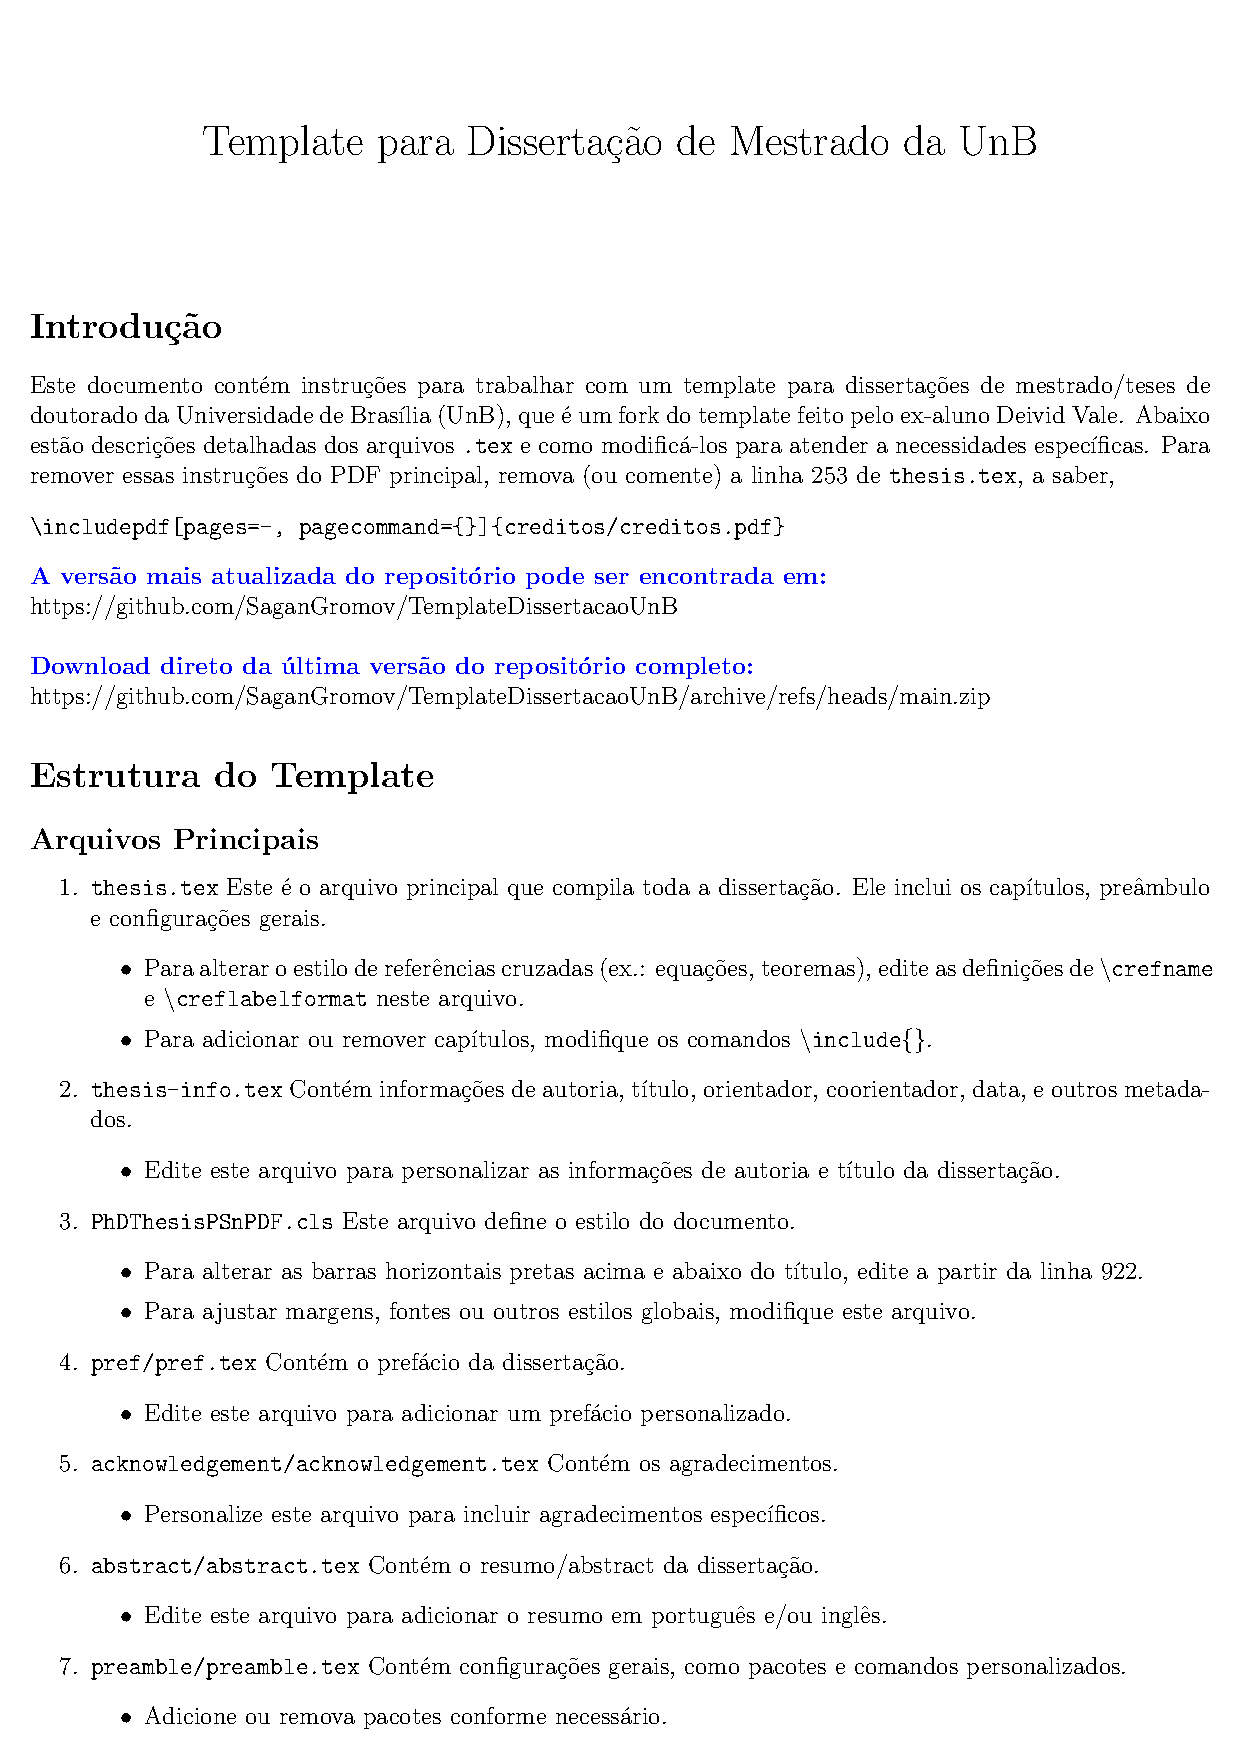
\includepdf[pages=-, pagecommand={}]{creditos/creditos.pdf}
\end{verbatim}
{\color{blue}\textbf{A versão mais atualizada do repositório pode ser encontrada em:}} \newline 
\href{https://github.com/SaganGromov/TemplateDissertacaoUnB}{https://github.com/SaganGromov/TemplateDissertacaoUnB}
\newline\newline
{\color{blue}\textbf{Download direto da última versão do repositório completo:}} \newline
\href{https://github.com/SaganGromov/TemplateDissertacaoUnB/archive/refs/heads/main.zip}{https://github.com/SaganGromov/TemplateDissertacaoUnB/archive/refs/heads/main.zip}


\section*{Estrutura do Template}

\subsection*{Arquivos Principais}

\begin{enumerate}
    \item \textbf{\texttt{thesis.tex}}  
    Este é o arquivo principal que compila toda a dissertação. Ele inclui os capítulos, preâmbulo e configurações gerais.  
    \begin{itemize}
        \item Para alterar o estilo de referências cruzadas (ex.: equações, teoremas), edite as definições de \texttt{\textbackslash crefname} e \texttt{\textbackslash creflabelformat} neste arquivo.
        \item Para adicionar ou remover capítulos, modifique os comandos \texttt{\textbackslash include\{\}}.
    \end{itemize}

    \item \textbf{\texttt{thesis-info.tex}}  
    Contém informações de autoria, título, orientador, coorientador, data, e outros metadados.  
    \begin{itemize}
        \item Edite este arquivo para personalizar as informações de autoria e título da dissertação.
    \end{itemize}

    \item \textbf{\texttt{PhDThesisPSnPDF.cls}}  
    Este arquivo define o estilo do documento.  
    \begin{itemize}
        \item Para alterar as barras horizontais pretas acima e abaixo do título, edite a partir da linha 922.
        \item Para ajustar margens, fontes ou outros estilos globais, modifique este arquivo.
    \end{itemize}

    \item \textbf{\texttt{pref/pref.tex}}  
    Contém o prefácio da dissertação.  
    \begin{itemize}
        \item Edite este arquivo para adicionar um prefácio personalizado.
    \end{itemize}

    \item \textbf{\texttt{acknowledgement/acknowledgement.tex}}  
    Contém os agradecimentos.  
    \begin{itemize}
        \item Personalize este arquivo para incluir agradecimentos específicos.
    \end{itemize}

    \item \textbf{\texttt{abstract/abstract.tex}}  
    Contém o resumo/abstract da dissertação.  
    \begin{itemize}
        \item Edite este arquivo para adicionar o resumo em português e/ou inglês.
    \end{itemize}

    \item \textbf{\texttt{preamble/preamble.tex}}  
    Contém configurações gerais, como pacotes e comandos personalizados.  
    \begin{itemize}
        \item Adicione ou remova pacotes conforme necessário.
        \item Defina comandos personalizados para uso em toda a dissertação.
    \end{itemize}

    \item \textbf{\texttt{assets/codigo\_segunda\_pagina/sec.tex}}  
    Este arquivo é usado para compilar a segunda página da dissertação, que geralmente contém informações institucionais e de apresentação.  
    \begin{itemize}
        \item Edite este arquivo para personalizar o conteúdo da segunda página, como título, autor, data e membros da banca.
        \item Certifique-se de que ele está incluído corretamente no arquivo \texttt{thesis.tex} com o comando:
        \begin{verbatim}
        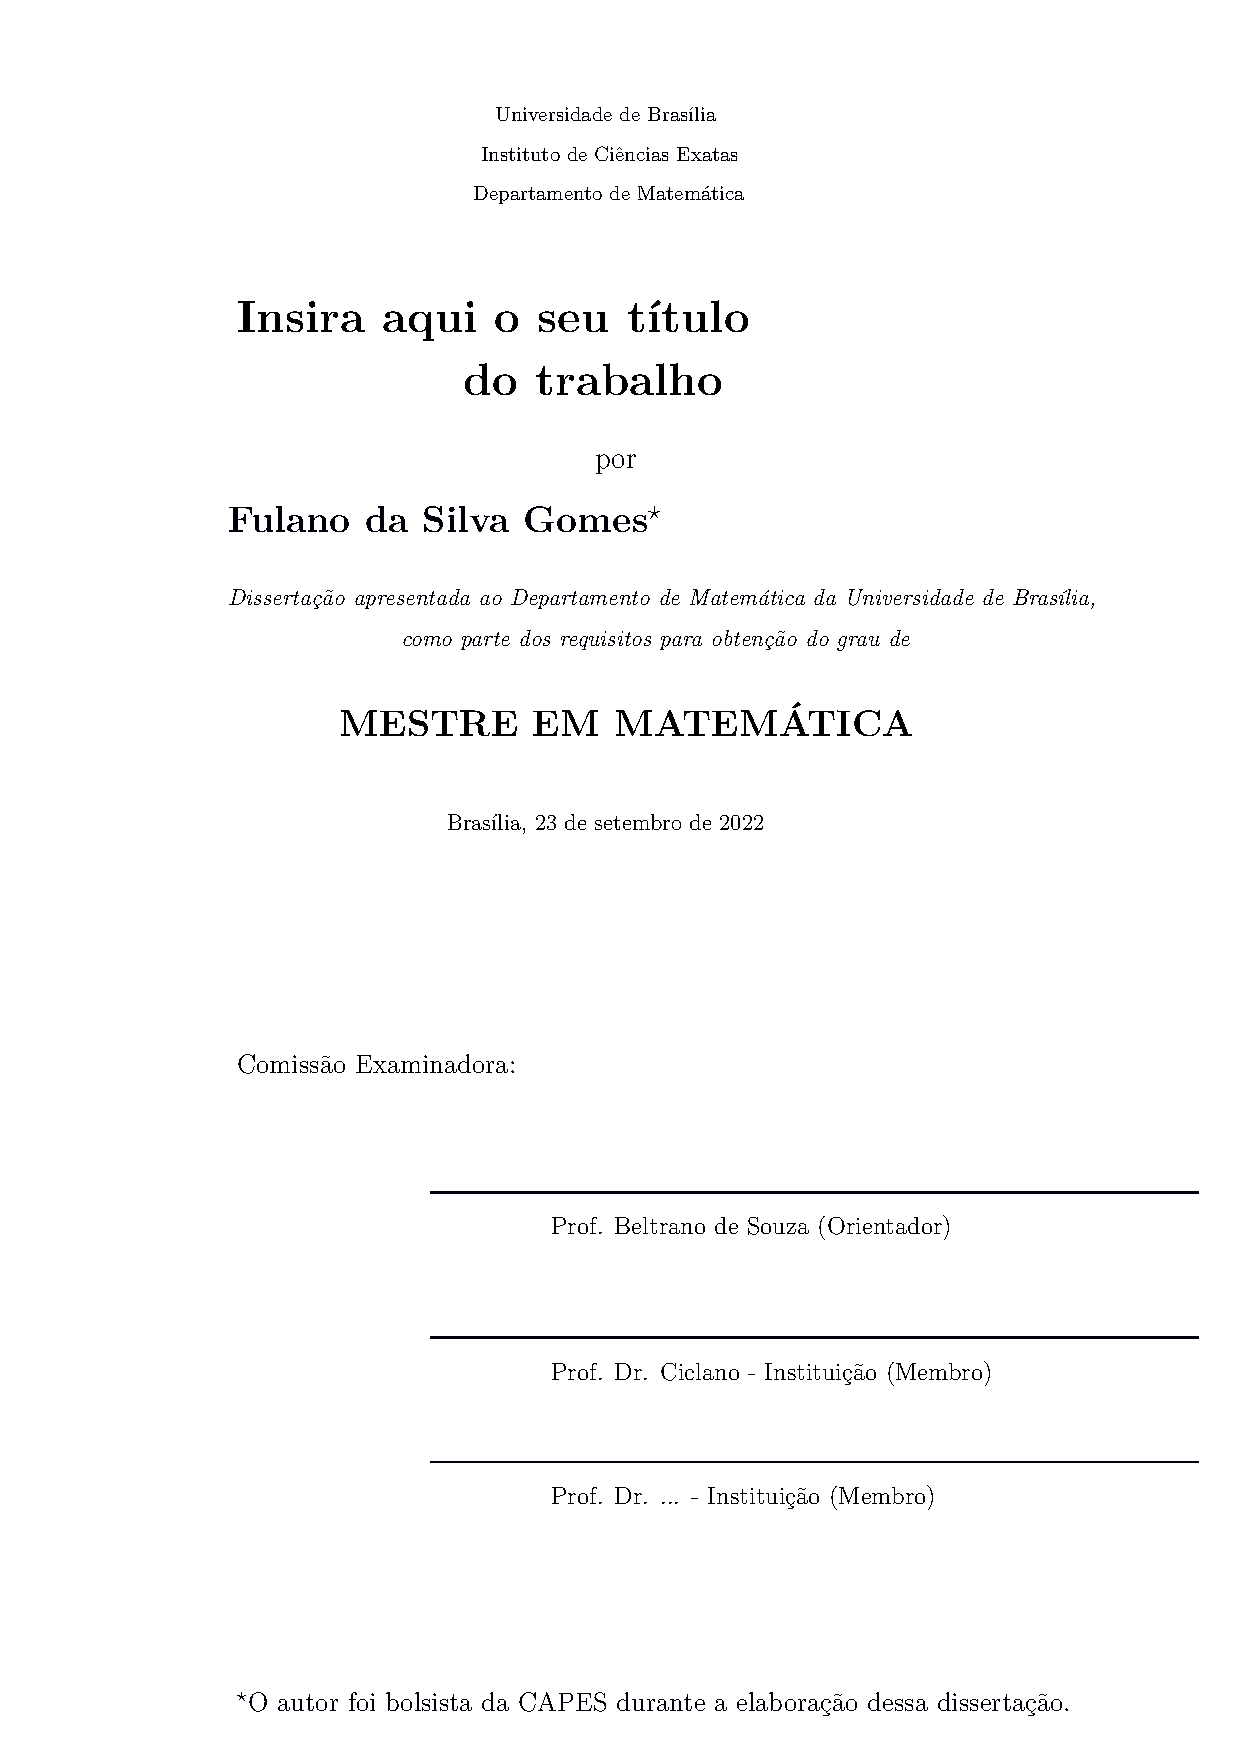
\includepdf[pages=1, pagecommand={{}}]{assets/codigo_segunda_pagina/sec.pdf}
        \end{verbatim}
    \end{itemize}
\end{enumerate}

\section*{Capítulos e Seções}

Os capítulos estão organizados em subdiretórios separados:
\begin{itemize}
    \item \textbf{\texttt{chapter\_1/chapter\_1.tex}} - Primeiro capítulo
    \item \textbf{\texttt{chapter\_2/chapter\_2.tex}} - Segundo capítulo
    \item \textbf{\texttt{chapter\_n/chapter\_n.tex}} - Capítulos adicionais
\end{itemize}

Para incluir ou remover capítulos, modifique os comandos \texttt{\textbackslash include\{\}} no arquivo \texttt{thesis.tex}. Por exemplo:
\begin{verbatim}
%!TEX root = ../thesis.tex
%*******************************************************************************
%*********************************** First Chapter *****************************
%*******************************************************************************
%\addtocounter{page}{7}
\fancypagestyle{plain}{%              '
\fancyhf{}
%\renewcommand{\subsectionmark}[1]{%
  %\markright{\MakeUppercase{\thesubsection\ \ \ \ #1 }}}
  %\renewcommand{\chaptermark}[1]{\markboth{teste ##1}{}}
  %\renewcommand{\sectionmark}[1]{\markright{\thesection\ ##1}}
  %\renewcommand{\headrulewidth}{0.7pt}
    %\fancyhead[LO]{\bfseries  \nouppercase{CAPÍTULO \thechapter}  }
        \fancyfoot[RO]{\bfseries Página \thepage \ de \pageref*{LastPage}}
    %\fancyhead[RO]{\bfseries \nouppercase \leftmark}
    }

\fancypagestyle{MyFancy}{%              
\fancyhf{}
%\renewcommand{\subsectionmark}[1]{%
  %\markright{\MakeUppercase{\thesubsection\ \ \ \ #1 }}}
  %\renewcommand{\chaptermark}[1]{\markboth{##1}{}}
  %\renewcommand{\sectionmark}[1]{\markright{\thesection\ ##1}}
  %\renewcommand{\headrulewidth}{0.7pt}
  \color{gal}
  \renewcommand{\sectionmark}[1]{ \markright{\textcolor{gal}{##1}}}
  \renewcommand\headrule{%

 \color{\corcaps}\noindent\makebox[\linewidth]{\rule{\paperwidth}{1pt}}
}
  \renewcommand\footrule{%

 \color{\corcaps}\noindent\makebox[\linewidth]{\rule{\paperwidth}{1pt}}
}
	%\fancyhead[RO]{\bfseries \rightmark}
	\fancyhead[LO]{\textcolor{gal}{\bfseries \nouppercase{\thesubsection} }}
    \fancyhead[RO]{\textcolor{gal}{\bfseries \nouppercase{\rightmark}}}
    \fancyfoot[RO]{\textcolor{gal}{\bfseries Página \thepage \ de \pageref*{LastPage}}}
    %\fancyfoot[LO]{\bfseries CAPÍTULO \thechapter}
    %\fancyhead[RO]{\bfseries \nouppercase \leftmark}
    }
\pagestyle{MyFancy}
\color{gal}
\chapter{Preliminary Concepts and Notations}
\markboth{Preliminaries}{Concepts}  
\label{cap:preliminares}



\ifpdf
    \graphicspath{{Chapter1/figs/Raster/}{Chapter1/figs/PDF/}{Chapter1/figs/}}
\else
    \graphicspath{{Chapter1/figs/Vector/}{Chapter1/figs/}}
\fi
%********************************** %First Section  **************************************

\PlaceText{69mm}{39mm}{ \color{gal}\noindent\makebox[\linewidth]{\rule{2\paperwidth}{1pt}}}

\PlaceText{69mm}{79mm}{ \color{gal}\noindent\makebox[\linewidth]{\rule{2\paperwidth}{1pt}}}

\color{black}


The purpose of this chapter is to establish the foundational concepts, notations, and conventions that will be used throughout this work. While we aim to make the exposition as self-contained as possible, some familiarity with basic concepts in Riemannian geometry and differentiable manifolds is assumed. Below, we provide a brief overview of the key ideas.

\section{Riemannian Manifolds}
\PlaceText{15mm}{13mm}{ \color{white}\noindent\makebox[\linewidth]{\rule{2\paperwidth}{10pt}}}
\vspace{-1.5cm}
\begin{oobs}
This section introduces the basic definitions and properties of Riemannian manifolds, including the notions of metric tensors, tangent spaces, and smooth maps. We also discuss the importance of coordinate charts and local frames in understanding the geometry of manifolds.
\end{oobs}

\begin{oobs}
We adopt standard notations for Riemannian geometry. For instance, the metric tensor is denoted by \( g \), and the Levi-Civita connection is denoted by \( \nabla \). The curvature tensor, Ricci tensor, and scalar curvature are also introduced with their respective notations.
\end{oobs}

\begin{deff}
A Riemannian manifold is a differentiable manifold \( \mathcal{M} \) equipped with a smooth, positive-definite metric tensor \( g \). This metric allows us to define notions of angles, lengths, and volumes on \( \mathcal{M} \).
\end{deff}

\begin{teorema}[Fundamental Theorem of Riemannian Geometry]
On a Riemannian manifold \( (\mathcal{M}, g) \), there exists a unique torsion-free connection \( \nabla \) that is compatible with the metric \( g \). This connection is called the Levi-Civita connection.
\end{teorema}

\begin{demm}
The proof involves verifying the existence and uniqueness of the Levi-Civita connection using the Koszul formula.
\end{demm}

\section{Tensors}
\vspace{-0.7cm}
This section provides an overview of tensor algebra and calculus, focusing on the types of tensors commonly encountered in Riemannian geometry. Topics include tensor products, contractions, and the metric-induced isomorphisms between tensors of different types.

\begin{deff}
A tensor of type \( (r, s) \) on a vector space \( V \) is a multilinear map \( T: V^* \times \cdots \times V^* \times V \times \cdots \times V \to \mathbb{R} \), where \( V^* \) is the dual space of \( V \).
\end{deff}

\begin{oobs}
Tensors can be represented in a chosen basis, and their components transform according to specific rules under a change of basis. This property makes tensors coordinate-independent objects.
\end{oobs}

\begin{proposicao}
The space of tensors of type \( (r, s) \) on a vector space \( V \) is a finite-dimensional vector space. Its dimension depends on the dimension of \( V \) and the values of \( r \) and \( s \).
\end{proposicao}

\section{Differential Forms}
Differential forms are a special class of tensors that are completely antisymmetric. They play a central role in integration on manifolds and in the formulation of Stokes' theorem.

\begin{deff}
A differential form of degree \( k \) on a manifold \( \mathcal{M} \) is a completely antisymmetric tensor field of type \( (0, k) \).
\end{deff}

\begin{namedthm}{Theorem}[Stokes' Theorem]
Let \( \mathcal{M} \) be an oriented manifold with boundary \( \partial \mathcal{M} \), and let \( \omega \) be a compactly supported \( (n-1) \)-form on \( \mathcal{M} \). Then,
\[
\int_{\mathcal{M}} d\omega = \int_{\partial \mathcal{M}} \omega.
\]
\end{namedthm}

\section{Additional Topics}
This section briefly introduces advanced topics such as the Hodge star operator, Laplacians, and Bochner's formula, which are essential tools in modern Riemannian geometry.

\begin{deff}
The Hodge star operator \( \star \) maps \( k \)-forms to \( (n-k) \)-forms on an \( n \)-dimensional Riemannian manifold. It is defined such that
\[
\alpha \wedge \star \beta = g(\alpha, \beta) \, \mathrm{vol},
\]
where \( \mathrm{vol} \) is the volume form.
\end{deff}

\begin{teorema}[Bochner's Formula]
On a Riemannian manifold, the Laplacian of a function \( f \) satisfies
\[
\Delta f = \text{div}(\nabla f),
\]
where \( \Delta \) is the Laplace-Beltrami operator.
\end{teorema}

\begin{demm}
The proof involves expressing the Laplacian in local coordinates and using the properties of the Levi-Civita connection.
\end{demm}
%!TEX root = ../thesis.tex
%*******************************************************************************
%****************************** Second Chapter *********************************
%************************f*******************************************************
%\addtocounter{page}{7}
\pagestyle{MyFancy}
\color{gal}
\chapter{O fluxo de Ricci}
\label{cap:OFLUXO}

\PlaceText{69mm}{35mm}{ \color{gal}\noindent\makebox[\linewidth]{\rule{2\paperwidth}{1pt}}}

\PlaceText{69mm}{79mm}{ \color{gal}\noindent\makebox[\linewidth]{\rule{2\paperwidth}{1pt}}}

\PlaceText{15mm}{13mm}{ \color{white}\noindent\makebox[\linewidth]{\rule{2\paperwidth}{10pt}}}

\color{black}

O conteúdo deste capítulo foi substituído por texto genérico para preservar a confidencialidade do trabalho original. A seguir, apresentamos uma visão geral genérica sobre o fluxo de Ricci.

\section{Motivação e exemplos}

O fluxo de Ricci é uma ferramenta matemática poderosa usada para estudar a geometria e a topologia das variedades. Ele foi introduzido por Richard Hamilton na década de 1980 e desempenhou um papel crucial na prova da Conjectura de Poincaré por Grigori Perelman.

\subsection{Definição do fluxo de Ricci}

O fluxo de Ricci é descrito pela seguinte equação diferencial parcial:
\[
\frac{\partial g_{ij}}{\partial t} = -2 \, \mathrm{Ric}_{ij},
\]
onde \( g_{ij} \) é a métrica Riemanniana e \( \mathrm{Ric}_{ij} \) é o tensor de Ricci associado.

\subsection{Propriedades gerais}

O fluxo de Ricci pode ser interpretado como uma deformação da métrica Riemanniana ao longo do tempo, suavizando irregularidades na curvatura da variedade. Ele é frequentemente comparado à equação do calor, que distribui uniformemente a temperatura em um objeto.

\section{Sólitons de Ricci}

Os sólitons de Ricci são soluções especiais do fluxo de Ricci que evoluem apenas por difeomorfismos e mudanças de escala. Eles desempenham um papel importante no estudo de singularidades do fluxo.

\subsection{Definição de sólitons}

Um sóliton de Ricci é uma solução da forma:
\[
\mathrm{Ric} + \nabla^2 f = \lambda g,
\]
onde \( f \) é uma função suave, \( \lambda \) é uma constante, e \( g \) é a métrica Riemanniana.

\subsection{Classificação de sólitons}

Os sólitons de Ricci podem ser classificados em três tipos:
\begin{itemize}
    \item \textbf{Shrinking}: \( \lambda > 0 \)
    \item \textbf{Steady}: \( \lambda = 0 \)
    \item \textbf{Expanding}: \( \lambda < 0 \)
\end{itemize}

\section{Singularidades no fluxo de Ricci}

As singularidades são um aspecto fundamental do estudo do fluxo de Ricci. Elas ocorrem quando a curvatura da métrica se torna infinita em tempo finito.

\subsection{Tipos de singularidades}

As singularidades podem ser classificadas em diferentes tipos, dependendo do comportamento da curvatura:
\begin{itemize}
    \item \textbf{Tipo I}: A curvatura cresce de forma controlada.
    \item \textbf{Tipo II}: A curvatura cresce de forma mais rápida e descontrolada.
\end{itemize}

\subsection{Resolução de singularidades}

Para lidar com as singularidades, técnicas como o "blow-up" são usadas para analisar o comportamento local da métrica perto do ponto de singularidade.

\section{Aplicações do fluxo de Ricci}

O fluxo de Ricci tem aplicações em várias áreas da matemática e da física. Ele é usado para estudar a geometria das variedades, resolver problemas em topologia e até mesmo em teorias físicas como a relatividade geral.

\subsection{Conjectura de Poincaré}

A aplicação mais famosa do fluxo de Ricci foi na prova da Conjectura de Poincaré, um dos problemas do Milênio, resolvido por Grigori Perelman.

\subsection{Geometrização de Thurston}

O fluxo de Ricci também foi usado para abordar a Conjectura de Geometrização de Thurston, que generaliza a Conjectura de Poincaré para dimensões superiores.

\section{Conclusão}

O fluxo de Ricci é uma ferramenta poderosa que conecta a geometria, a análise e a topologia. Ele continua sendo uma área ativa de pesquisa, com muitas questões abertas e aplicações potenciais.

\end{verbatim}

Cada capítulo pode conter suas próprias figuras, tabelas e referências bibliográficas locais.

\section*{Instruções para Incluir Teoremas, Observações e Outros Elementos}

Os estilos para teoremas, observações, definições e outros elementos estão definidos nos arquivos \newline \texttt{preamble/preamble.tex}, \texttt{preamble/config.tex} e \texttt{preamble/notation.tex}. Abaixo estão exemplos de como utilizá-los:

\subsection*{Teoremas}
\begin{verbatim}
\begin{teorema}
Seja $\mm^3$ uma variedade diferenciável fechada. Então $\mm^3$ é homeomorfa a $\mathbb{S}^3$.
\end{teorema}
\end{verbatim}

\subsection*{Observações}
\begin{verbatim}
\begin{oobs}
Este resultado é uma consequência direta do Teorema de Poincaré.
\end{oobs}
\end{verbatim}

\subsection*{Definições}
\begin{verbatim}
\begin{deff}
Uma métrica Riemanniana é uma função que associa a cada ponto de uma variedade um produto interno no espaço tangente.
\end{deff}
\end{verbatim}

\subsection*{Proposições}
\begin{verbatim}
\begin{proposicao}
Sejam $a, b \in \mathbb{R}$. Então $a + b = b + a$.
\end{proposicao}
\end{verbatim}

\subsection*{Lemas}
\begin{verbatim}
\begin{lema}
Se $f$ é uma função contínua em um intervalo fechado, então $f$ é limitada.
\end{lema}
\end{verbatim}

\subsection*{Corolários}
\begin{verbatim}
\begin{col}
Se $\mm^3$ é simplesmente conexa e compacta, então $\mm^3$ é homeomorfa a $\mathbb{S}^3$.
\end{col}
\end{verbatim}

\subsection*{Perguntas}
\begin{verbatim}
\begin{pergunta}
Quais são todas as topologias possíveis de uma superfície compacta?
\end{pergunta}
\end{verbatim}

\subsection*{Exemplos}
\begin{verbatim}
\begin{exem}
O toro $\mathbb{T}^2 = \mathbb{S}^1 \times \mathbb{S}^1$ é um exemplo de uma superfície compacta.
\end{exem}
\end{verbatim}

\section*{Personalização de Notação}

Os comandos personalizados para notação matemática estão definidos em \texttt{preamble/notation.tex}. Exemplos de comandos disponíveis:

\begin{itemize}
    \item \textbf{Produto de Kulkarni-Nomizu}: \texttt{\textbackslash KN}
    \item \textbf{Divergência}: \texttt{\textbackslash divv}
    \item \textbf{Curvatura Escalar}: \texttt{\textbackslash Scal}
    \item \textbf{Ricci}: \texttt{\textbackslash Ric}
    \item \textbf{Curvatura Riemanniana}: \texttt{\textbackslash Rm}
\end{itemize}

Exemplo de uso:
\begin{verbatim}
A curvatura escalar é denotada por $\Scal$, enquanto a curvatura de Ricci é $\Ric$.
\end{verbatim}

\end{document}
